\let\negmedspace\undefined
\documentclass{beamer}
\mode<presentation>
\usepackage{amsmath}
\usepackage{amssymb}
%\usepackage{advdate}
\usepackage{adjustbox}
\usepackage{subcaption}
\usepackage{multicol}
\usepackage{mathtools}
\usepackage{listings}
\usepackage{url}
\def\UrlBreaks{\do\/\do-}
\usetheme{Madrid}
\usecolortheme{lily}
\setbeamertemplate{footline}
{
	\leavevmode%
	\hbox{%
		\begin{beamercolorbox}[wd=\paperwidth,ht=2.25ex,dp=1ex,right]{author in head/foot}%
			\insertframenumber{} / \inserttotalframenumber\hspace*{2ex} 
		\end{beamercolorbox}}%
		\vskip0pt%
	}
\setbeamertemplate{navigation symbols}{}

\providecommand{\nCr}[2]{\,^{#1}C_{#2}} % nCr
\providecommand{\nPr}[2]{\,^{#1}P_{#2}} % nPr
\providecommand{\mbf}{\mathbf}
\providecommand{\pr}[1]{\ensuremath{\Pr\brak{#1}}}
\providecommand{\qfunc}[1]{\ensuremath{Q\brak{#1}}}
\providecommand{\sbrak}[1]{\ensuremath{\left[#1\right]}}
\providecommand{\lsbrak}[1]{\ensuremath{\left[#1\right.}}
\providecommand{\rsbrak}[1]{\ensuremath{\left.#1\right]}}
\providecommand{\brak}[1]{\ensuremath{\left(#1\right)}}
\providecommand{\lbrak}[1]{\ensuremath{\left(#1\right.}}
\providecommand{\rbrak}[1]{\ensuremath{\left.#1\right)}}
\providecommand{\cbrak}[1]{\ensuremath{\left\{#1\right\}}}
\providecommand{\lcbrak}[1]{\ensuremath{\left\{#1\right.}}
\providecommand{\rcbrak}[1]{\ensuremath{\left.#1\right\}}}
\theoremstyle{remark}
\newtheorem{rem}{Remark}
\newcommand{\sgn}{\mathop{\mathrm{sgn}}}
\providecommand{\abs}[1]{\left\vert#1\right\vert}
\providecommand{\res}[1]{\Res\displaylimits_{#1}} 
\providecommand{\norm}[1]{\lVert#1\rVert}
\providecommand{\mtx}[1]{\mathbf{#1}}
\providecommand{\mean}[1]{E\brak{ #1 }}
\providecommand{\fourier}{\overset{\mathcal{F}}{ \rightleftharpoons}}
%\providecommand{\hilbert}{\overset{\mathcal{H}}{ \rightleftharpoons}}
\providecommand{\system}{\overset{\mathcal{H}}{ \longleftrightarrow}}
%\newcommand{\solution}[2]{\textbf{Solution:}{#1}}
%\newcommand{\solution}{\noindent \textbf{Solution: }}
\providecommand{\dec}[2]{\ensuremath{\overset{#1}{\underset{#2}{\gtrless}}}}
\newcommand{\myvec}[1]{\ensuremath{\begin{pmatrix}#1\end{pmatrix}}}
\let\vec\mathbf

\lstset{
	%language=C,
	frame=single, 
	breaklines=true,
	columns=fullflexible
}

\numberwithin{equation}{section}

\title{10.4.ex.13.1: Finding Roots of a Quadratic}
\author{EE24BTECH11018 - Durgi Swaraj Sharma}
\date{}

\begin{document}

\frame{\titlepage}

%-------------------------------
\begin{frame}
\frametitle{Problem Statement}
\textbf{Find the roots of the quadratic equation:}
\begin{align}
3x^2 - 5x + 2 = 0
\end{align}
We will use two methods:\\
\quad Newton-Raphson Method\\
  \quad Eigenvalue Approach via QR Decomposition \brak{\text{using Householder Reflections}}
\end{frame}

%-------------------------------
\begin{frame}
\frametitle{Newton-Raphson Method: Overview}
\textbf{Idea:} Iteratively improve an initial guess to find a root of $f\brak{x}=0$.

\textbf{Iteration Formula:}
\begin{align}
x_{n+1} = x_n - \frac{f\brak{x_n}}{f'\brak{x_n}}
\end{align}

\textbf{For our equation:}
\begin{align}
f\brak{x} &= 3x^2 - 5x + 2,\quad f'\brak{x} = 6x - 5\\[1mm]
\Rightarrow \quad x_{n+1} &= x_n - \frac{3x_n^2 - 5x_n + 2}{6x_n - 5}.
\end{align}
\end{frame}

%-------------------------------
\begin{frame}
\frametitle{Newton-Raphson Method: How It Works}
\begin{itemize}
	\item Start with an initial guess $x_0$.
	\item Compute the function value $f\brak{x_n}$ and its derivative $f'\brak{x_n}$.
	\item Update the guess using:
	\begin{align}
	x_{n+1} = x_n - \frac{f\brak{x_n}}{f'\brak{x_n}}
	\end{align}
	\item Repeat until the guess converges to a root.
\end{itemize}
\textbf{Key Points:}
\begin{itemize}
	\item Requires a good initial guess.
	\item Convergence is rapid if the guess is close to the actual root.
	\item May fail or converge slowly if the derivative is small or the guess is poor.
\end{itemize}
\end{frame}

%-------------------------------
\begin{frame}
\frametitle{QR Decomposition via Householder Reflections: Overview}
\textbf{Goal:} Decompose a matrix $A$ into $A = QR$, where:
\begin{itemize}
	\item $Q$ is an orthogonal matrix.
	\item $R$ is an upper triangular matrix.
\end{itemize}
  This is useful for finding eigenvalues \brak{\text{the roots of the characteristic equation}} using the QR algorithm.
\end{frame}

%-------------------------------
\begin{frame}
\frametitle{Householder Reflections: The Concept}
\textbf{Householder Reflection:} A transformation that reflects a vector about a hyperplane.

\textbf{Reflection Matrix:}
\begin{align}
H = I - 2\frac{vv^T}{v^T v},
\end{align}
where $v$ is a vector chosen such that when $H$ is applied to a vector, it zeros out all but the first component.
\end{frame}

%-------------------------------
\begin{frame}
\frametitle{Using Householder Reflections for QR Decomposition}
\begin{enumerate}
	\item \textbf{Select a column:} For the $k$th column of $A$ starting from row k, choose vector $a_k$.
	\item \textbf{Construct vector $v$:}
	\begin{align}
	v = a_k + \text{sign}\brak{a_{k1}}\,\norm{a_k}\,e_1,
	\end{align}
	where $e_1$ is the standard basis vector.
	\item \textbf{Form the Householder matrix:}
	\begin{align}
	H_k = I - 2\frac{vv^T}{v^T v}.
	\end{align}
	\item \textbf{Apply transformation:} Compute
	\begin{align}
    A^{\brak{k}} = H_k\,A^{\brak{k-1}},
	\end{align}
	so that the subdiagonal elements in the $k$th column are zeroed.
	\item \textbf{Accumulate $Q$:} The product of the Householder matrices gives
	\begin{align}
	Q^T = H_m\,H_{m-1}\,\cdots\,H_1,
	\end{align}
	so that $Q = H_1\,H_2\,\cdots\,H_m$.
\end{enumerate}

\end{frame}

%-------------------------------
\begin{frame}
\frametitle{QR Algorithm for Eigenvalue Computation}
\begin{itemize}
	\item Once $A$ is decomposed as $A = QR$, form a new matrix:
	\begin{align}
	A_{1} = RQ.
	\end{align}
\item $A_1$ is similar to $A$ \brak{\text{same eigenvalues}}.
	\item Repeat the QR decomposition on $A_{1}$ to obtain $A_{2}$, and so on.
	\item After sufficient iterations, $A_k$ converges to an upper triangular \brak{Schur} form.
	\item The eigenvalues are the diagonal entries of the converged matrix.
\end{itemize}
\end{frame}

%-------------------------------
\begin{frame}
\frametitle{Application to the Quadratic Equation}
\textbf{Companion Matrix:} For $3x^2 - 5x + 2 = 0$, first normalize to get a monic polynomial:
\begin{align}
x^2 - \frac{5}{3}x + \frac{2}{3} = 0.
\end{align}
The companion matrix is:
\begin{align}
C = \begin{bmatrix}
0 & \frac{2}{3} \\
1 & -\frac{5}{3}
\end{bmatrix}.
\end{align}
\begin{itemize}
  \item Applying the QR algorithm \brak{\text{using Householder reflections}} on $C$ yields its eigenvalues.
	\item The eigenvalues are the roots of the quadratic: approximately $0.666667$ and $1.000000$.
\end{itemize}
\end{frame}

%-------------------------------
\begin{frame}
\frametitle{Summary}
\begin{block}{Newton-Raphson Method}
	\begin{itemize}
		\item Iterative scheme:
		\begin{align}
		x_{n+1} = x_n - \frac{f\brak{x_n}}{f'\brak{x_n}}.
		\end{align}
		\item Converges rapidly with a good initial guess.
	\end{itemize}
\end{block}

\begin{block}{QR Decomposition via Householder Reflections}
	\begin{itemize}
		\item Uses reflections to zero out subdiagonal entries.
    \item Decomposes $A$ into $Q$ \brak{\text{orthogonal}} and $R$ \brak{\text{upper triangular}}.
		\item The QR algorithm applied to the companion matrix finds the eigenvalues.
	\end{itemize}
\end{block}
Both methods confirm the roots:
\begin{align}
x \approx 0.666667 \quad \text{and} \quad x \approx 1.000000.
\end{align}
\end{frame}

\begin{frame}
  \frametitle{Plot}
  \begin{figure}
    \centering
    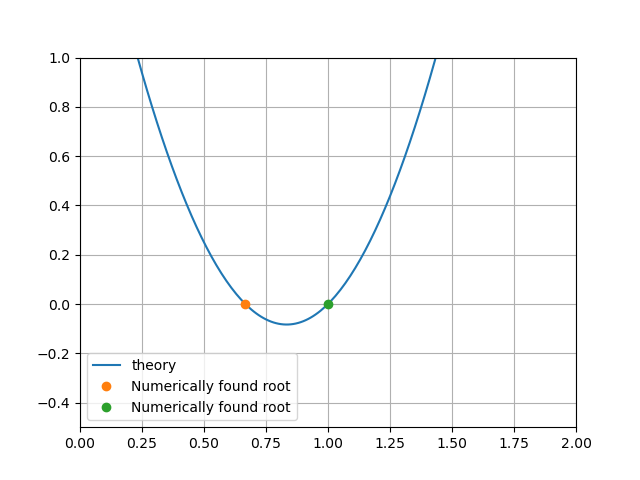
\includegraphics[width=0.8\columnwidth]{figs/fig.png}
    \caption{Plotting the result from Newton-Raphson method}
  \end{figure}
\end{frame}

\end{document}

